\documentclass{article}
\usepackage[left=2cm,right=2cm,top=2cm,bottom=2cm]{geometry}
\usepackage[utf8]{inputenc}
\usepackage[german]{babel}
\usepackage{amsmath}
\usepackage{dsfont}
\usepackage[export]{adjustbox}
\usepackage{amsthm}
\usepackage{color}
\usepackage{amsfonts}
\usepackage{amssymb}
\usepackage{wasysym}
\usepackage{makeidx}
\usepackage{graphicx}
\usepackage[colorlinks=true,urlcolor=blue,linkcolor=blue]{hyperref}
\usepackage{ziffer}
\usepackage{minted}
\usepackage{xcolor}
\usepackage{framed}
\usepackage{mdframed}
\usepackage{subfiles}
\usemintedstyle{emacs}

\definecolor{purp}{HTML}{9A72AC}
\definecolor{re}{HTML}{FC6255}
\definecolor{gre}{HTML}{83C167}
\definecolor{blu}{HTML}{58C4DD}
\definecolor{shadecolor}{rgb}{0.85,0.85,0.85}
\definecolor{bg}{rgb}{0.95,0.95,0.95}
\setlength{\parindent}{0em} 

\BeforeBeginEnvironment{minted}{\begin{mdframed}[linewidth =2 ,backgroundcolor=bg , linecolor=black, linewidth=0.5]}
\AfterEndEnvironment{minted}{\end{mdframed}}

\newtheorem{defi}{Definition}
\BeforeBeginEnvironment{defi}{\begin{mdframed}[linewidth =2 ,backgroundcolor=bg , linecolor=black, linewidth=0.5]}
\AfterEndEnvironment{defi}{\end{mdframed}}

\newcommand{\bsp}{\textbf{Beispiel}:}
%\newcommand{\task}{\textbf{Aufgabe}:}

\newcommand{\bol}[1]{\textbf{#1}}
\newcommand{\q}[1]{\glqq #1\grqq}
\newcommand{\DODO}[1]{\textbf{\textcolor{red}{DODO:}} #1 \\ \begin{center}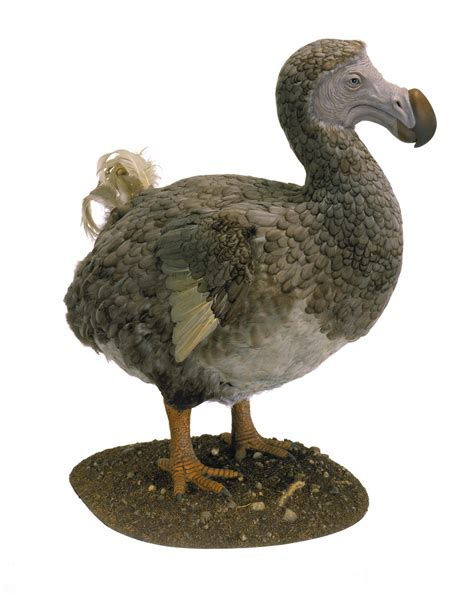
\includegraphics[scale=0.2]{../../media/dodo.jpg} \end{center}}

\newenvironment{task}[1]{
    \begin{shaded*}
    \textbf{Aufgabe #1}:
}{
    \end{shaded*}
}

\begin{document}
Man unterscheidet im Wesentlichen zwei große Untertypen von Listenimplementierungen. Die, die sich auf Felder (arrays) stützen und
die, die eine \q{verzeigerte} Struktur aufweisen (linked lists). Da Felder bereits aus der zehnten Jahrgangsstufe bekannt sind, ist dieser Ansatz der naheliegenderer und wir beginnen mit ihm. 
Für den Moment wollen wir uns ein Feld als reservierten Speicherplatz vorstellen, im Folgenden symbolisiert durch
eine Aneinanderreihung an Quadraten. Aktuell soll das Feld noch vollständig leer sein.
\begin{center}
    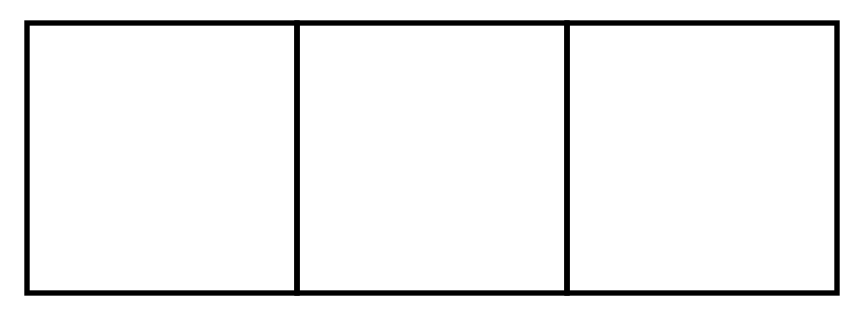
\includegraphics[scale=0.15]{../../media/empty_arr.png}
\end{center}
In Java werden Felder allerdings standardmäßig mit 0 bzw. null intialisiert, wenn keine weiteren Vorgaben gemacht werden.
\bsp
\begin{minted}{Java}
    int[] array = new int[3];
\end{minted}
Die Variable array zeigt nun zu einem Feld, das 3 mal den Eintrag 0 enthält, 
in Java-Schreibweise: $\{0,0,0\}$ \\

\begin{center}
    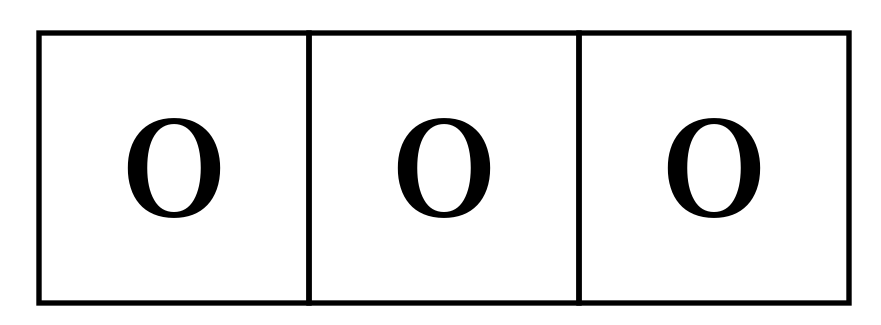
\includegraphics[scale = 0.15]{../../media/zero_arr.png}
\end{center}

Neben primitiven Datentypen wie int können auch Listen von beliebigen Objekten gebildet werden. Nehmen wir an, wir haben
eine Klasse \q{Mensch }bereits erzeugt, dann wird

\begin{minted}{Java}
    Human[] humans = new Human[5];
\end{minted}

ein Feld mit 5 Einträgen null erzeugen, auf das durch die Variable humans zugegriffen wird. \\
Wir können auf beliebige Einträge eines zuvor erzeugten Feldes zugreifen, wenn wir Zugriff auf die Variable haben, die den Anfang der Liste speichert, z.B.:
\begin{minted}{Java}
    int[] numbers = {5,3,42,17,-2};
    int thirdEntry = numbers[2];
    System.out.println(thirdEntry);
\end{minted}

Der obige Code wird die Zahl 42 auf die Konsole schreiben. Dieses Beispiel soll daran erinnern, dass
in der Informatik bei 0 zu zählen begonnen wird. Auf den für uns dritten Eintrag wird also mit der 
\q{2} zugegriffen. \\

Versuchen wir stattdessen, z.B. mit humans[0] auf den ersten Menschen zuzugreifen, werden wir nur null erhalten,da dieses Feld aktuell nur null-Einträge enthält. 

\begin{center}
    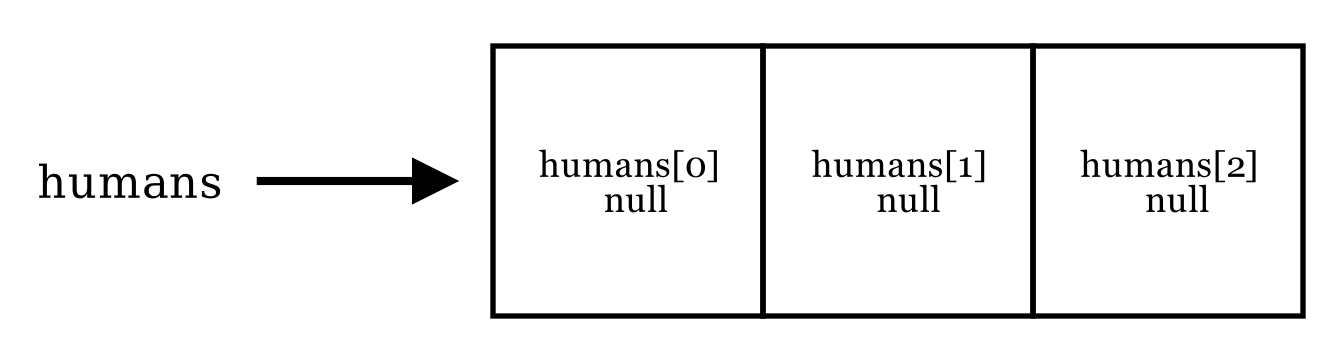
\includegraphics[scale=0.2]{../../media/queue_humans_null.png}
\end{center}

Haben wir die Methode hintenAnfügen() (push()) implementiert und drei Menschen Anna, Berti und Christo 
erzeugt und zur Warteschlange hinzugefügt: 

\begin{center}
    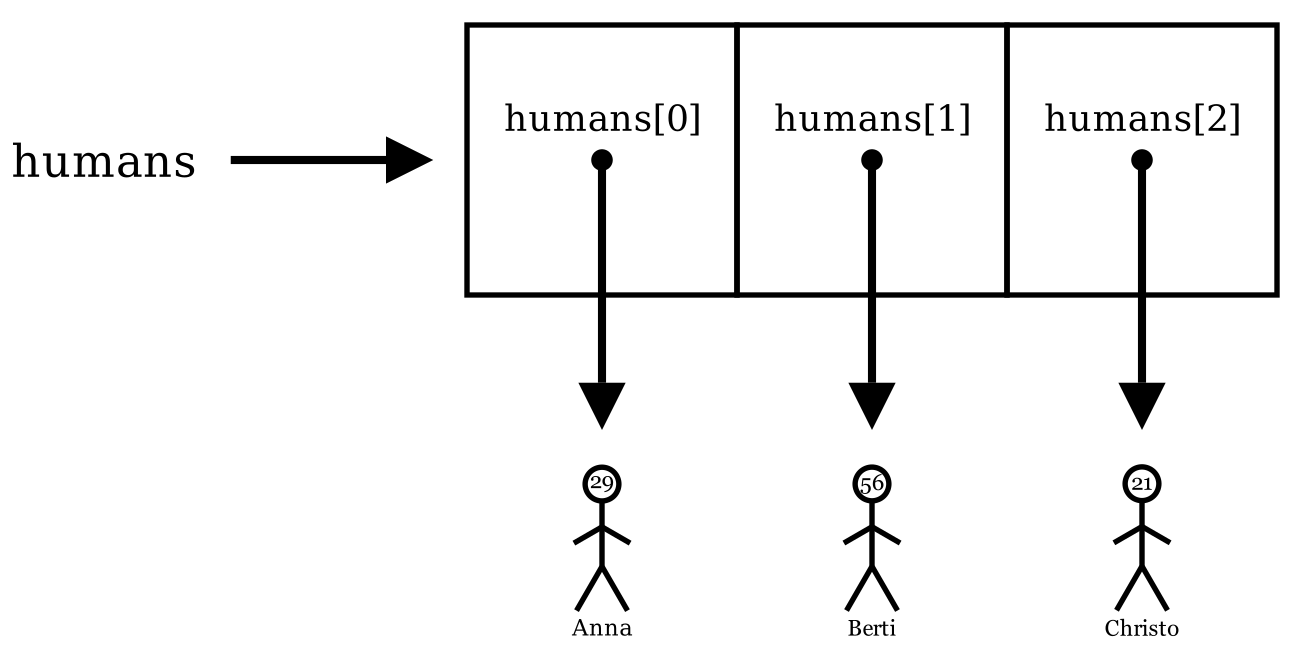
\includegraphics[scale=0.2]{../../media/queue_humans_arrows.png}
\end{center}
Dabei stehen die Strichys (\href{https://www.youtube.com/watch?v=xVmGb7qACfA&t}{Germanistik-Exkurs}) ebenfalls wieder für eine bestimmte Menge an Daten, die (ggf. an ganz anderer physikalischer Stelle) im Speicher abgelegt sind. \\ 
Grundsätzlich bietet das Feld an sich in seiner üblichen Implementierung in Java bereits alle Eigenschaften, die wir 
von einer Liste verlangen würden. Wenn unsere Warteschlange benutzt wird, soll aber nur am Anfang 
entnommen und am Ende angefügt werden können. Es ist also mehr Kontrolle nötig. \\
Beginnen wir damit unsere Warteschlange als neue Klasse zu definieren. Da es unser Ziel ist eine Schlange von Menschen zu modellieren, brauchen wir zunächst eine Klasse, die einen Menschen beschreibt. 

\begin{center}
    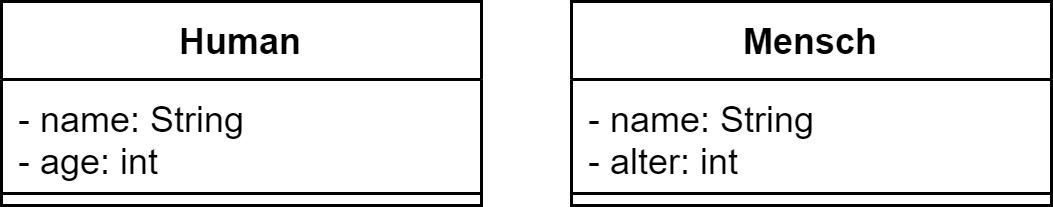
\includegraphics[scale=0.25]{../../media/human.png}
\end{center}

Bevor es mit der Implementierung weitergeht bietet sich an dieser Stelle eine Wiederholung der wichtigsten drei Diagrammarten an, die in der Oberstufe Verwendung finden:
\begin{itemize}
    \item Klassendiagramm
    \item Objektdiagramm
    \item Sequenzdiagramm
\end{itemize}
$\Rightarrow$ Exkurs im \textbf{Anhang}


\begin{minted}{Java}
    public class Human() {
        private String name;
        private int age; 
    
        public Human(String name, int age){
            this.name = name;
            this.age = age;
        }
    }
\end{minted}
Unsere Menschen haben aktuell nur die Attribute Name und Alter und außer dem Konstruktor sind keine weiteren
Methoden vorhanden. Unser Ziel ist es eine Warteschlange der folgenden Struktur zu bauen: \\
\begin{center}
    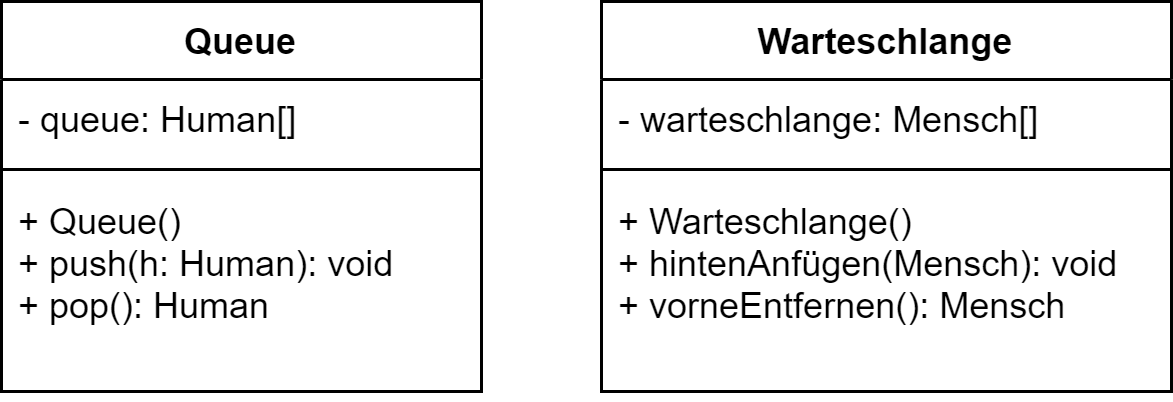
\includegraphics[scale=0.25]{../../media/queue_diagramm.png}
\end{center}

\begin{minted}{Java}
    public class MyListArray(){
        private Human[] queue;
        private int count;

        public MyListArray() {
            queue = new Human[5];
            count = 0;
        }
    }
\end{minted}
Der Konstruktor erzeugt ein neues Feld der Größe 5 und setzt die derzeitige Belegung auf 0. Die Anzahl der 
Menschen in der Warteschlange muss nicht zwangsläufig in einem Attribut gespeichert werden, da es aber eine 
Größe ist, die häufiger von Nutzen ist, wäre eine ständige Berechnung unnötiger Aufwand.  \\
Um die Warteschlange auch sinnvoll verwenden zu können müssen weitere Methoden ergänzt werden. Wir beginnen mit der hintenAnfügen() Methode. Da wir spezifizieren müssen, was wir anfügen wollen folgt für die Signatur:
\begin{minted}{Java}
    public void push(Human humanToAdd) 
\end{minted}
Ein erster - naiver - Ansatz zur Befüllung wäre der folgende: 
\begin{minted}{Java}
    public void push(Human humanToAdd) {
        for(int i = 0; i < queue.length; i++) {
            if(queue[i] == null) {
                queue[i] = humanToAdd;
                break;
            }
        }
    }
\end{minted}

\begin{task}{1}
Begründe Sie kurz, warum diese Implementierung ineffizient ist. 
\end{task}
\vspace{2cm}
Eine effizientere Lösung besteht darin, das Attribut $anzahl$ zu verwenden, dadurch vereinfacht sich die Implementierung zu: 

\begin{minted}{Java}
    public class MyListArray(){
        private Human[] queue;
        private int count; 

        public MyListArray() {
            queue = new Human[5];
            count = 0;
        }

        public void push(Human humanToAdd) {
            queue[count] = humanToAdd;
            count++;
        }
    }
\end{minted}

\begin{task}{2}
Begründen Sie, warum auch diese Implementierung noch problematisch ist. Lösen Sie das Problem!
\end{task}

\vspace{2cm}

Aktuell kann unsere Liste nur fünf Elemente enthalten. Versucht man ein sechstes Element anzuhängen, so erhält man
als Nachricht \textbf{\q{java.lang.ArrayIndexOutOfBoundsException}}. Es wird also versucht an eine Position der Liste einzufügen, die nicht existiert.\\
Ist die Liste voll, muss das Feld vergrößert werden. Da dies eine Funktionalität ist, die wir eventuell noch an anderer Stelle brauchen könnten, ist es sinnvoll dafür eine eigene Methode anzulegen. Sie erzeugt ein neues, größeres Feld und kopiert die Einträge aus dem alten Feld in das neue Feld. Anschließend wird neu verzeigert.\\
\textit{Erinnerung:} Die Länge eines Feldes ist in einem öffentlichen Attribut des Felds gespeichert, auf das direkt zugegriffen wird, $length$ ist deswegen kein Methodenaufruf in untenstehendem Code, sondern bezieht sich auf dieses Attribut. Keine Klammern!
\begin{minted}{Java}
    public void push(Human humanToAdd) {
        if(count == queue.length) {
            enlargeArray();
        } 
        queue[count] = humanToAdd;
        count++;
    }

    private void enlargeArray() {
        Human[] newQueue = new Human[queue.length + 5];
        for(int i = 0; i < queue.length; i++){
            newQueue[i] = queue[i];
        }
        queue = newQueue;
    }
\end{minted}

Um die Methode effizienter zu gestalten, wird das Feld um 5 Plätze vergrößert. Man möchte zu große
Felder vermeiden (insbesondere mit leeren Einträgen!), um nicht unnötig Speicherplatz zu verschwenden (die Implementierung der ArrayList, die von Java direkt angeboten wird verwendet z.B. eine Vergrößerung um 5 Plätze, für Details zu dieser \q{vorgebauten} Struktur siehe \href{https://docs.oracle.com/en/java/javase/17/docs/api/java.base/java/util/ArrayList.html#add(E)}{Java Doc ArrayList}). \\
Als nächstes muss noch das vorderste Element der Warteschlange entfernt werden können. Spätestens
hier zeigt sich, dass das Feld für diese Anwendungsform der Liste nur schlecht geeignet ist. Wenn  
das vorderste Element entfernt wird, müssen alle folgenden Elemente einen Platz nach vorne geschoben werden, ansonsten entsteht mit der Zeit ein großer Block an leeren Einträgen im Feld. 
Dieser Kopiervorgang nimmt vergleichsweise viel Zeit und Leistung in Anspruch. Eine mögliche Implementierung
der Methode sieht folgendermaßen aus:

\begin{minted}{Java}
    public Human pop() {
        if(queue[0] == null) {
            return null;
        }
        Human toReturn = queue[0];
        for(int i = 0; i < count - 1; i++){
            queue[i] = queue[i+1];
        }
        queue[count-1] = null;
        count--;
        return toReturn;    
    }
\end{minted}

Die Methode gibt eine Referenz auf das entfernte Objekt zurück, sofern es existiert. Wird diese Referenz nicht in einer neuen 
Variable gespeichert bei Anwendung der Methode, so wird sie vom garbage collector aufgeräumt und ist 
vollständig verschwunden. Alternativ könnte auch eine äquivalente Methode mit der Signatur \\

\begin{minted}{Java}
    public void pop()
\end{minted}
definiert werden. In diesem Fall wird der erste Mensch aus der Schlange entfernt und das Objekt geht \q{verloren}. \\
Visualisierung der Anfügen und Entfernen-Methoden: \href{https://youtu.be/e_XY3wmY02M}{Youtube - push - pop} \\

\textbf{Übungsblock} \\
Die folgenden Aufgaben steigen grob im Schwierigkeitsgrad an und erweitern die Funktionalität der 
Liste sukzessive. Die Lösungen finden sich kommentiert auf den darauf folgenden Seiten. Versuchen Sie die beschriebenen Methoden zunächst selbst zu implementieren!

\begin{task}{3}
Schreiben Sie eine Methode schreibeListe (printList()), die die Warteschlange in einer sinnvollen Weise 
auf der Konsole sichtbar macht. \\
Hinweis: Ergänzen Sie eine passende Methode in der Klasse Mensch (Human)!
\end{task}

\begin{task}{4}
Schreiben Sie eine Methode menschAnPosition(int position) (humanAtPosition(int position)), die eine 
Referenz zum Menschen an der angegebenen Position zurückgibt. Beachten Sie Grenz- bzw. Spezialfälle!
\end{task}

\begin{task}{5}
    Schreiben Sie eine Methode sucheMenschInSchlange(Mensch m) (searchHumanInQueue(Human h)), die die Position 
    des Menschen in der Schlange zurückgibt. \\
    \textit{Hinweis}: Überschreiben Sie die allgemeine equals() Methode in der Klasse Mensch.
\end{task}

\begin{task}{6}
    Schreiben Sie eine Methode enthält(Mensch m) (contains(Human h)), die wahr zurückgibt, wenn 
    der der entsprechende Mensch in der Schlange ist, anderfalls falsch. \\
    \textit{Hinweis}: Verwenden Sie die equals-Methode aus Aufgabe 5
\end{task}
\begin{task}{7}
    Schreiben Sie eine Methode entferneAnPosition(int position) (removeAtPosition(int position)), die den 
    Menschen an der gegebenen Stelle entfernt und die übrigen nach vorne rutschen lässt. \\
    Schreiben Sie zwei Versionen dieser Methode, eine, die den Menschen nur entfernt und eine, die 
    eine Referenz zu diesem Menschen zurückgibt.
\end{task}

\begin{task}{8 - für Experten}
    Schreiben Sie eine Methode zusammenfügen(MeineListeFeld zweiteWarteschlange) (concatenate(MyListArray secondQueue)),
    die eine zusammengefügte Liste zurückgibt. 
\end{task}

\begin{task}{9 - für Experten}
    Schreiben Sie eine Methode fügeSortiertHinzu(Mensch m) (appendSorted(Human h)), die die Warteschlange nicht 
    von hinten auffüllt, sondern die Menschen an einer bestimmten Stelle einsortiert. \\
    \textit{Hinweis}: Dazu muss eine Vergleichsmethode in der Klasse Mensch definiert werden. Z.B. könnte nach Alter, oder auch nach 
    Namen oder nach einer Kombination von beidem sortiert werden. 
\end{task}

\begin{task}{10 - frei}
    Überlegen Sie sich eigene, sinnvolle weitere Methoden für die Warteschlangen-Implementierung.
\end{task}

\end{document}